\documentclass[a4paper,11pt]{article}
\usepackage{graphicx,listings,float,geometry, amsmath,placeins}
%\usepackage[firstpage]{draftwatermark}
%\SetWatermarkLightness{0.5}
%\SetWatermarkScale{4}
\setcounter{tocdepth}{2}
\usepackage[dutch]{babel}
\usepackage{xspace, color,mdframed}
\usepackage[usenames,dvipsnames]{xcolor}
\newcommand{\protoref}{sectie \ref{sec:protocol}}
\newcommand{\bericht}[1]{
{\begin{center}

\colorbox{YellowGreen!20}{\makebox[\textwidth][c]{{
\textsc{#1}
}}}
\end{center}
}}
\newcommand{\udp}{\textsc{udp}\xspace}
\newcommand{\tcp}{\textsc{tcp}\xspace}
\geometry{
	includeheadfoot,
	margin=2.54cm
}

\begin{document}
	\begin{titlepage}
	\begin{center}
		
		{\Huge Informele Specificatie \\[0.5cm]OGO 2.3 - Multiplayer Game}\\[0.5cm]
		\rule{\linewidth}{0.5mm}\\[0.5cm]
				\bigskip
		\huge \textit{``Grudge of the Oblivious''}
		
		{\Large
		Luca van Ballegooijen, Tim van Dalen, \\
		Carl van Dueren den Hollander, Peter Koymans,\\
		Kay Lukas en Ferry Timmers\\[1cm]
		}
		
		{\large
		OGO 2.3\\
		Groep 3 \\[1cm]
		Faculteit Wiskunde en Informatica\\
		Technische Universiteit Eindhoven\\[1cm]
		}
		
		\begin{abstract}

    In dit document zullen we de kritieke punten bij dit project identificeren. Vervolgens bekijken we de taken die bij dit project een rol spelen. Tenslotte zullen we dit gebruiken om een werkplan voor het project op te stellen.
\end{abstract}


		\vfill

		{\large \today}
	\end{center}
\end{titlepage}

	
	\tableofcontents
	\newpage

	\section{Introductie}
	Informatici in de hedendaagse wereld komen vaak in aanraking met het ontwerpen van complexe programma's. Complexe programma's hebben vaak ook een netwerk aspect en een grafische aspect. Zelfs bij technische programma's, die vaak minder grafisch intensief zijn, als matlab worden al deze aspecten verenigd. Dit drukt de noodzaak uit dat elke informaticus basiskennis heeft van computergrafiek, computernetwerken en het ontwerpen van complexe programma's. Al deze aspecten worden verenigd in dit project: \textsc{ogo} 2.3 - Nethunt. Dit document ligt ... INSERT MORE

Voor dit project werd ons gevraagd om een interactief, gedistribueerd 3D-spel te ontwikkelen. Dit houdt in dat elk speler lokaal dezelfde spelsituatie heeft, en deze op het scherm van de speler worden afgebeeld. Natuurlijk kan de afbeelding op het scherm verschillen per speler. Een andere eis was dat er voedsel aanwezig moet zijn. E\'en van de randvoorwaarden was dat elke speler ... INSERT MORE
	\newpage

    \section{Beschrijving onderdelen}
    Wij verdelen het programma in drie zoveel mogelijk onafhankelijke onderdelen. Hierbij onderscheiden wij:
    \begin{itemize}
    \item Een onderdeel die het communiceren naar andere spelers mogelijk maakt;
	\item Het model van de sc\`ene. Denk hierbij aan de staat, locatie en grafische modellen van gebouwen, spelers en het terrein;
	\item De gebruikersomgeving die de interactie van de speler met het spel mogelijk maakt en ook het grafische model weergeeft tijdens het spel.
    \end{itemize}

    Als uitgangspunt ontwerpen wij de verschillende onderdelen zodanig dat elk van de onderdelen zo onafhankelijk mogelijk ontwikkeld kunnen worden.
    	
    \subsection{Protocol module}
    De protocol module is het onderdeel die het mogelijk maakt om:
	\begin{itemize}
	\item Een nieuw spel op te starten. Het spel komt dan in de zogenaamde opstart fase. Andere spelers kunnen dan aan dit spel meedoen, ze komen dan in de lobby van dat spel;
	\item De lijst van alle spellen, die nog in de opstart fase zijn, in het subnet van de computer weer te geven;
	\item Mee te doen met een bestaand spel dat nog in de opstart fase zit;
	\item Het spel te beginnen;
	\item Mutaties van de staat van het spel te ontvangen en te versturen.
	\end{itemize}
	De manier, waarop deze communicatie verloopt, is beschreven vanaf \protoref. De gebruikersomgeving kan de protocol module een opdracht geven. Deze opdracht zal dan asynchroon worden uitgevoerd door de protocol module. Dit betekent dat het protocol uit zichzelf berichten kan ontvangen en verwerken. Door middel van threads wordt er voor gezorgd dat het protocol de taken onafhankelijk kan uitvoeren.
	
    \subsection{Het model van de sc\`ene}
    Het model van de sc\`ene vervult twee rollen. Het houdt de huidige staat van het spel bij en zorgt ervoor dat de huidige staat van het spel afgebeeld kan worden op het scherm. Het model is dus in principe een passief element, het zal niet uit zichzelf acties uitvoeren (uitzonderingen daargelaten). Een diepgaande beschrijving van het model kan gevonden worden in sectie \ref{sec:model}

    \subsection{Gebruikersomgeving}
   	De gebruikersomgeving moet zowel het grafische model van het spel afbeelden op het scherm als de interactie van de speler via het toetsenbord en muis afhandelen. Ook moet de gebruikersomgeving het mogelijk maken voor de gebruiker om een spel op te starten of mee te doen aan een spel in de opstart fase.

    \subsubsection{De opzet van het spel}
    Tijdens de opzet van het spel zal de gebruikersomgeving een venster weer moeten geven met alle spellen in het subnet van de computer. De gebruiker kan dan kiezen om mee te doen aan een van deze spellen of zijn eigen spel te openen. Als de gebruiker zelf een spel opent, kunnen andere gebruikers in hetzelfde subnet ook meedoen aan dit spel. Deze spelers kunnen dan met elkaar communiceren in een lobby. Hierin kunnen zij ook aangeven of zij klaar zijn om het spel te starten. Zodra alle gebruikers hebben aangegeven dat zij klaar zijn, kan het spel worden gestart. De keuze om het spel te starten is dan aan de gebruiker, die ook het spel heeft geopend.

    \subsubsection{Tijdens het spel}
    De gebruikersomgeving zal tijdens het spel via \textsc{openGL} de lokale staat van het spel afbeelden op het scherm. Dit wordt gedaan door de \emph{render} methode van het object \emph{World} aan te roepen, die is beschreven in sectie \ref{sec:model}. De gebruikersomgeving zal daarna alleen nog menu's, mogelijke kaarten en informatie als de sterkte van het harnas en de hoeveelheid geld op het scherm moeten aangeven (zoals beschreven in het document Informele Beschrijving). Door de 2D-modus van openGL te gebruiken kan dit gemakkelijk getekend worden boven op de grafische representatie van de wereld.

	De gebruikersomgeving zal ook het model aanpassen aan de hand van de interactie van de gebruiker met de omgeving. Om dit voor elkaar te krijgen slaat de gebruikersomgeving alle muisbewegingen, klikken en toetsenbord aanslagen op en past het model op de bijbehorende manier aan. Een verdere uitleg van de interactie tussen de gebruikersomgeving en het model is gegeven in appendix \ref{sec:interactscenmodel}.

    \section{Onderlinge samenhang}
    De drie onderdelen, die wij hierboven beschreven hebben, moeten natuurlijk allemaal met elkaar kunnen communiceren. Deze communicatie zullen we nu beschrijven.

    \subsection{Gebruikersomgeving en protocol module tijdens de opzet van het spel}
    De gebruikersomgeving en de protocol module communiceren tijdens de opzet van het spel compleet asymmetrisch. Dat wil zeggen dat het protocol op elk moment een bericht kan sturen naar de gebruikersomgeving en ook andersom. Om dit mogelijk te maken, heeft de protocol module verschillende functies ge\"implementeerd, die aangeroepen kunnen worden door de gebruikersomgeving. Deze kunnen bijvoorbeeld gebruikt worden om een nieuw spel aan te maken of mee te doen aan een bestaand spel. Op deze manier kan de gebruikersomgeving acties van de gebruiker omzetten in een actie van het protocol: de protocol module handelt dit dan af.

    De protocol module luistert actief naar binnenkomende berichten. Aangezien het protocol real-time verplichtingen heeft, zal de module gebruik maken van meerdere threads. Zo fungeert de module los van de gebruikersomgeving. Als er een bijzondere gebeurtenis heeft plaatsgevonden, kan het protocol dit doorgeven aan de gebruikersomgeving door middel van zogenaamde \emph{call-backs}. Dit zijn methoden die de gebruikersomgeving implementeert, zodat de protocol module informatie kan doorgeven aan de gebruikersomgeving. De gebruikersomgeving zal deze informatie zodanig moeten afhandelen dat het afgebeeld kan worden op het scherm.

    Niet alle communicatie van de protocol module en de gebruikersomgeving verloopt via call-backs en methoden, sommige informatie zal de protocol module namelijk niet als een gebeurtenis doorgeven. Deze informatie wordt louter opgeslagen in de protocol module en kan de gebruikersomgeving opvragen. Denk hierbij aan de lijst van spellen op het subnet, spelers in het spel, enzovoorts. Een voorbeeld van interactie van de gebruikersomgeving en protocol module is gegeven in een \textsc{msc} in appendix \ref{app:MSCLobbyCon}.

    \subsection{Model van de sc\`ene en de gebruikersomgeving tijdens het spel}
    Het model van de sc\`ene zal niet actief communiceren met de gebruikersomgeving tijdens het spel. Dat wil zeggen dat er geen asymmetrische communicatie plaatsvindt via call-backs. De gebruikersomgeving zal aan de hand van de invoer van de gebruiker het model aanpassen. De gebruikersomgeving zal ook de grafische representatie van de staat van het spel uit het model halen. Het model maakt dit mogelijk door de beschreven \emph{render} methode in de interface \emph{object}. Het model zorgt voor enkele globale methoden die in \'e\'en keer een actie van de gebruiker kan verwerken in het model. Hierdoor hoeft de gebruikersomgeving alleen een paar globale methoden aan te roepen. Hiermee voorkomen wij dat de gebruikersomgeving veel gebruik moet maken van de structuur van het model. Zo wordt de gebruikersomgeving minder afhankelijk van de implementatie van het model.

    \section{Gedetailleerde klassenbeschrijving}
    De sc\`ene zullen wij beschrijven aan de hand van een klassendiagram, dit bespreken we op een \emph{top-down} manier. Het klassendiagram zelf is toegevoegd in appendix A.3. Een aantal basisklassen, zoals $Point2d, Point3d$ en $Vector3d$, zijn hierin voor de overzichtelijkheid niet aangegeven. We maken bovendien de afspraak dat de types $Percentage/Power/Time/Duration$ vrij kunnen worden gebruikt. Deze kunnen bijvoorbeeld \emph{Reals} of \emph{Integers} zijn, afhankelijk van de implementatie. We zijn nu klaar om de gebruikte interfaces te bespreken.

\subsection{Interfaces}
Er zijn twee interfaces in het klassendiagram: de zogenaamde $Object$ interface en $BoundingObject$ interface. We geven het implementeren van een interface aan door $\langle\langle$ interface naam$\rangle \rangle$ voor de naam van de klasse, die de interface implementeert.  De klasse Object bevat een aantal standaard attributen om de conversie tussen globale en lokale co\"ordinaten te bewerkstelligen. Dit zijn $origin, yaw, patch$ en $roll$. Hier zijn de hoeken yaw, pitch en roll in graden tussen 0 en 360. 0 is in dit geval inclusief, 360 is exclusief.

Bovendien bevat Object nog het attribuut $children$, dit is een array van Objects. De reden hiervoor is dat dit hi\"erarchisch modelleren mogelijk maakt. Vervolgens bevat Object nog een aantal methoden: $draw, render, prerender$ en $postrender$. De prerender methode zorgt voor de transformatie van globale co\"ordinaten naar lokale co\"ordinaten. De postrender methode zorgt voor de transformatie van lokale co\"ordinaten naar globale co\"ordinaten.

De draw methode zorgt voor het tekenen zelf. Deze methode is natuurlijk abstract gemaakt. De render methode combineert alle voorgaande methoden: het roept eerst prerender aan. Vervolgens wordt draw aangeroepen. Daarna wordt ook de draw functie van de Objects in de children array aangeroepen. Als laatste wordt nog postrender aangeroepen.

De interface BoundingObject is een subklasse van Object. De aard van deze type objecten is zodanig dat ze begrensd zijn. Hier hoort dus een corresponderende \emph{bounding box} bij. De bounding box staat in het attribuut bBox van het type BoundingBox. Ook in dit geval geldt dat de klasse BoundingBox niet in het klassendiagram is opgenomen voor de overzichtelijkheid.

De bounding box is niet alleen handig voor het tekenen. Het is namelijk ook mogelijk met deze bounding box te testen voor \emph{collisions}. Hier wordt getest of er een collision plaatsvindt van het object met de lijn gegeven door het startpunt origin en met richting direction. Het object zelf of een van de children wordt teruggeven in het geval van een collision. Als er geen collision is, dan zullen we \emph{null} teruggeven. Dit kan bijvoorbeeld gebruikt worden bij het schieten.

\subsection{Model van de sc\`ene}
    \label{sec:model}
We zijn nu klaar om de klassen, die worden gebruikt om de sc\`ene te modelleren, te bespreken.  Al deze klassen implementeren de interface BoundedObject. Merk op dat de klasse Object dus niet gebruikt wordt, behalve dat BoundedObject een subklasse hiervan is. Deze klasse kan echter nuttig zijn voor verdere uitbreiding van het spel. We beginnen met de $World$ klasse. Deze bevat een attribuut $homePlayer$ van het type $Player$. Dit attribuut wordt gebruikt om de speler zelf te identificeren.

De $walkHomePlayer$ wordt gebruikt door de speler om rond te lopen door de wereld. Er wordt dan periodiek een bericht naar alle andere spelers gestuurd om dit door te geven. Verder wordt de $walk$ functie van Player aangeroepen, deze functie wordt verderop nog besproken. De $yesno$ boolean wordt gebruikt om aan te geven of de speler moet lopen of stoppen met lopen. De $shootHomePlayer$ heeft een vergelijkbare interpretatie.

De $buildBuilding$ wordt gebruikt door de speler om een nieuw gebouw neer te zetten. Hiervoor moet natuurlijk een punt worden aangegeven op de grond en het gewenste gebouw. Het gewenste gebouw is dan van het type $Building$. Als laatste is er nog de functie $pickup$. Deze wordt gebruikt als een speler een object, zoals een muntje, opraapt. Merk op dat dit niet noodzakelijk de speler zelf hoeft te zijn. Opraapbare objecten zijn van het type $Droppable$.

\subsubsection{Het terrein}
$World$ heeft een $Terrain$, die het terrein van de sc\`ene voorstelt. Het terrein wordt gemodelleerd door een grid. De methode $groundCollision$ wordt gebruikt bij het bouwen van een gebouw. In deze methode wordt berekend welke cel van de grid is aangeklikt. Merk op dat de cellen van de grid worden aangeklikt met behulp van het vizier en dat het vizier altijd in de huidige kijkrichting staat. Voor groundCollision kan dus de huidige locatie en kijkrichting worden gebruikt.

De methode $getHeight$ geeft de hoogte van het terrein voor een zekere cel terug. Op dit moment is ons terrein in principe nog vlak, maar dit willen we later nog uitbreiden. Als we het terrein hoogte willen geven, is een mogelijke optie om dit in de grid op te slaan. Aangezien het terrein nu nog vlak is, is dit nog niet opgenomen in het klassendiagram: hiervoor is slechts een simpele en kleine uitbreiding nodig.

Terrain heeft een array van Droppables en een matrix van $Structures$. Droppable stelt een opraapbaar object voor: dat is nu alleen nog een muntje. Een opraapbaar object heeft een zekere waarde. Bovendien zal een opraapbaar object na een zekere tijd verdwijnen, hiervoor is het attribuut $dieTime$ van het type $Time$. Als laatste is er nog de methode $onPickup$. Deze methode werkt de staat van World bij na de actie die is veroorzaakt door het oppakken van een Droppable. Dus in het geval van een muntje wordt de hoeveelheid goud van het team verhoogd.

De klasse Structure is abstract: de klassen Mine en Building zijn de subklassen. In de klasse Mine wordt opgeslagen hoeveel inkomen deze mijn genereert in een zekere periode. Deze periode is vast voor alle mijnen. Hiervoor kunnen we dus een constante defini\"eren. De klasse Building is ook weer abstract. Een Building heeft altijd \'e\'en corresponderend team. Het heeft de attributen $cost, income, buildTime, buildDuration, attackPower$ en $health$.

Het attribuut $cost$ staat voor de totale kosten van het gebouw. $Income$ representeert het inkomen dat het gebouw genereert. Ook hier geldt dat de tijdseenheid vast is. $BuildTime$ representeert het moment waarop de speler de opdracht heeft gegeven het gebouw neer te zetten, $BuildDuration$ vertelt hoelang het bouwen duurt. Dit wordt gebruikt door de animatie van het gebouw. Het wordt verder gebruikt om te bepalen wanneer het neerzetten van het gebouw voltooid is.

$AttackPower$ geeft aan hoe ernstig het harnas wordt beschadigd, als het gebouw een speler neerschiet. $Health$ geeft de sterkte van het gebouw aan: als de health nul wordt, gaat het gebouw kapot. We merken op dat de attributen $income$ en attackPower geen betekenis hebben voor alle gebouwen. Zo heeft attackPower geen betekenis voor de resourceMine. Als dit het geval is, zal altijd de waarde 0 moeten worden gekozen voor dit attribuut.

De klasse $ResourceMine, DefenseTower$ en $HQ$ zijn subklassen van $Building$. Een ResourceMine is het gebouw dat over een $Mine$ kan worden geplaatst. Mine staat dus voor de delfplaats en ResourceMine voor de mijn. Een Mine hoeft dus in principe niet van een team te zijn, terwijl een ResourceMine dat altijd zal zijn.

\subsubsection{De speler en teams}
World heeft in principe twee $Teams$, deze klasse representeert de verschillende teams. Later kunnen we dit nog uitbreiden naar meer dan twee teams. Elk team heeft een zekere hoeveelheid goud in de kas. Dit wordt opgeslagen in het attribuut resources. Bovendien heeft Team een array van $Players$. Hierin staan natuurlijk de spelers van dat team.

De klasse Player modelleert een speler in het spel. In het attribuut $health$ wordt de sterkte van het harnas opgeslagen. Het attribuut $lastShoot$ representeert het laatste moment, waarop de speler heeft geschoten. Hierdoor kunnen we het spel uitbreiden, zodat de speler pas weer kan schieten na een zekere \emph{cooldown} periode. De methode $fireLaser$ verzorgt de animatie bij het schieten. Hiervoor wordt de klasse $Laserbeam$ gebruikt: deze klasse heeft een $fireTime$ en $fireDuration$. De fireTime is het moment van vuren. De fireDuration bepaalt dan hoe lang de animatie van het schot duurt. De methode $walk$ in Player zorgt voor de animatie als de speler loopt. Het $connectie$ attribuut maakt het mogelijk voor de $communicator$ klasse om de bijbehorende connectie van een speler op te kunnen vragen.

\subsubsection{De camera}
Als laatste heeft de World nog een $Camera$. We laten het nog open voor de implementatie welke attributen worden gebruikt om de camera te representeren. De klasse $Camera$ is een abstracte klasse. Een implementatie van $Camera$ heeft dus de verplichting dat een speler vanuit het juiste punt in de juiste richting kijkt. In principe implementeren wij camera alleen door de klasse PlayerCamera: deze camera bekijkt de wereld vanuit een derde persoonsperspectief. Andere implementaties zijn later nog mogelijk.

\subsection{Statische objecten}
Er is nog \'e\'en cruciaal statisch object voor de implementatie van het spel, waarvan de functies door alle andere klassen kunnen worden gebruikt. Dit is de klasse $Communicator$, die de communicatie met andere spelers verzorgt.  Voor een uitgebreide beschrijving van het protocol, zie \protoref. Met een boolean in deze klasse wordt aangegeven of dit proces de token heeft. Verder wordt opgeslagen wanneer de token voor het laatst is ontvangen. Hiervoor gebruiken we het type Date, die de huidige tijd representeert.

De klasse Communicator maakt gebruik van de klasse $Message$. De klasse Message representeert het bericht dat moet worden verzonden. Het heeft een attribuut type, die het soort bericht aangeeft. Dit attribuut is van het type $MessageType$, dat voor de overzichtelijkheid is weggelaten uit het klassendiagram. MessageType is immers een simpele enumeratie.

Verder heeft Message nog een boolean $requiresToken$, die aangeeft of de token vereist is om dit soort bericht te mogen versturen. De token wordt gebruikt voor mutual exclusion. Als laatste heeft het message nog een array van argumenten. Het type $Argument$ hangt af van de implementatie, hiervoor kan bijvoorbeeld string of array van bytes worden gekozen. Verder zijn er nog de methoden $addInteger, addReal, addString, addIntegers$ en $addReals$. Deze methoden voegen de type in de naam van de methode toe aan het bericht.

De methode $broadcastMessage$ stuurt een $message$ naar elke speler die deelneemt aan het spel. Als het bericht een token nodig heeft ($requiresToken = True$) dan wordt het bericht alleen verstuurd als Communicator ook het token heeft ($hasToken = True$). In het geval dat het bericht geen token nodig heeft, wordt het bericht meteen verstuurd. Als het bericht een token nodig heeft en de communicator heeft geen token, dan wordt het bericht niet verstuurd. Dan retourneert de methode ook false: later kan nog een keer worden geprobeerd. In het geval dat het bericht wel wordt verstuurd, dan retourneert de methode true.

Door middel van de methode $lockToken$ kan men afdwingen dat de token niet meer vrijgegeven wordt totdat $unlockToken$ wordt aangeroepen. De methode heeft \'e\'en parameter $BlockingWait$. Deze parameter geeft aan of de functie moet wachten totdat de communicator de token heeft of direct moet stoppen als de communicator de token niet heeft. Als de communicator niet kan locken omdat de token er nog niet is, retourneert de methode $false$. In elk ander geval wordt $true$ geretourneerd.

De methode $broadcastTeamMessage$ doet hetzelfde als $broadcastMessage$ behalve dat deze alleen berichten verstuurd naar spelers die in het team $t$ zitten.

    \section{Het berichtsformaat}
    \label{sec:protocol}
    We zijn nu klaar om het formaat van de berichten formeel te defini\"eren. Hiervoor gebruiken we BNF (\emph{Backus-Naur Form}):
	
	\begin{center} \boxed{\begin{aligned}
    <\textsc{message}> &::= <\textsc{command}> <\textsc{args}> <\textsc{crlf}> \\
    <\textsc{command}> &::= \text{``A''...``Z''} <\textsc{command}> | \text{``A''...``Z''} \\
    <\textsc{args}>    &::= \text{`` ''} | <\textsc{string}> | <\textsc{value}> <\textsc{args}> \\
    <\textsc{string}>  &::= \text{`` :''} <\text{printable characters}>^{*} \\
    <\textsc{value}>   &::= \text{`` ''}  <\text{graphical characters}>^{*} \\
    <\textsc{crlf}>    &::= \textsc{cr lf}
    \end{aligned} }\end{center}

    Een bericht bestaat uit een commando met argumenten. Na het commando en argumenten komt het einde van de regel: \textsc{crlf}. Met ``A''...``Z'' bedoelen we een willekeurige hoofdletter. Een commando is dus een hoofdletter of een hoofdletter gevolgd door een commando. Hieruit volgt dat een commando een niet-lege reeks van hoofdletters is.

    Het argument van een commando is alleen een spatie, een string of een waarde gevolgd door een argument. Een string begint altijd met een spatie gevolgd door een dubbele punt. Vervolgens volgt een willekeurige reeks van ``printable characters''. Hiermee bedoelen we letters, cijfers en spaties. Een waarde begint ook altijd met een spatie. Daarna volgt een reeks van ``graphical characters''. Daarmee bedoelen we letters en cijfers.

    We merken nog op dat het mogelijk is om een bericht te sturen zonder argumenten. Dit kan wel degelijk nuttig zijn, aangezien er bijvoorbeeld ook informatie kan worden gehaald uit het commando zelf.

    Het onderscheid tussen een value en een string is dus klein. Een string is altijd het laatste onderdeel van een argument. Merk op dat de verschillende argumenten worden onderscheiden door spaties. Aangezien er nog een dubbele punt voor de string staat, mag een string wel spaties bevatten zonder dat hierdoor onze berichten meerdere betekenissen krijgen. Immers, zodra we een spatie gevolgd door een dubbele punt tegenkomen, kunnen we concluderen dat we aan het laatste argument zijn begonnen. Een spatie is dan onderdeel van het argument zelf en betekent dus niet dat een nieuw argument is begonnen. Op deze manier kunnen namen van spelers en de naam van het spel spaties bevatten.

    \section{De berichten}
    We zullen nu alle gebruikte berichten afgaan met een korte toelichting. Hierbij kijken we vooral naar het nut voor de ontvanger. Hiervoor gebruiken we een aantal conventies. We zullen voor de leesbaarheid komma's plaatsen tussen de verschillende argumenten. Deze zijn dus niet deel van het bericht. Ook zullen we de commando's laten eindigen met een punt, dit moet dan worden gelezen als \textsc{cr lf}.

    \subsection{Server detectie}
    Het \emph{Broadcast} bericht wordt gebruikt voor het detecteren van servers tijdens de initialisatie. Dit bericht word periodiek door servers verstuurd met behulp van broadcast over \udp. We hebben ervoor gekozen om dit bericht elke vijf seconden te sturen. De wachttijd voor de gebruikers is dan nog steeds verwaarloosbaar, terwijl het netwerk nauwelijks wordt belast.

    Spelers moeten continu voor deze Broadcast berichten scannen. De gevonden servers worden dan in een lijst gezet. De speler kan dan uit deze lijst van servers kiezen. Hierdoor kunnen processen in hetzelfde subnet een server vinden. We geven ook de mogelijkheid om direct het ip van de server op te geven. Dit heeft het grote voordeel dat het mogelijk wordt om ook te spelen met spelers buiten het lokale netwerk. Merk op dat de server natuurlijk alleen wordt gebruikt voor het opzetten van het spel.

    Het bericht bevat de versie van het spel en het huidige aantal spelers. Bovendien bevat het de naam van het spel. Het bericht heeft de volgende syntax:
    \bericht{GOTO, version, numPlayers :gameName.}

    \subsection{De lobby}
    Het \emph{Name} bericht wordt gebruikt na de server detectie. Als een speler de lobby van een bepaald spel wil binnengaan, wordt dit gedaan door een Name bericht te sturen. In dit bericht aan de server stuurt de speler zijn gewenste naam mee:
    \bericht{NAME :playername.}
    Indien de speler wordt toegelaten, zal de server een \emph{Hello} bericht terugsturen als reactie op het Name bericht (en wordt dus alleen gestuurd aan de speler die het Name bericht heeft gestuurd aan de server). Hierin staat het toegewezen ID van de speler, de versie, het aantal spelers en de naam van het spel. Dit geeft het volgende bericht:
    \bericht{HELLO, pid, version, numPlayers :gameName.}
    Na het versturen van het Hello bericht, zal de server ook meteen een aantal \emph{Player} berichten sturen. Dit bericht wordt aan de nieuwe speler gestuurd om het team en status van elke medespeler kenbaar te maken. De status kan B zijn voor niet ready, R zijn voor ready of H zijn voor host. Alle spelers zitten standaard in hetzelfde team. Bovendien hebben alle spelers standaard de status niet ready. Het spel kan pas beginnen als alle spelers ready zijn. Dan kan de speler, die de server draait, op start drukken om het spel te starten. Het bericht heeft de volgende syntax:
    \bericht{PLAYER, pid, tid, state :playerName.}
    Na het versturen van de Hello en Player bericht, zal de server aan alle spelers een \emph{Join} bericht sturen. Hierdoor weten alle spelers dat er een nieuwe medespeler is bijgekomen. Dit bericht wordt ook aan de nieuwe speler zelf gestuurd. Hierdoor kan de nieuwe speler concluderen dat de Player berichten zijn afgelopen. Dit bericht bevat de ID van de speler en de naam van de speler:
    \bericht{JOIN, pid :playerName.}
    Het \emph{Part} bericht wordt gestuurd als de verbinding van een speler met de server, al dan niet vrijwillig, wordt verbroken. Dit bericht wordt aan iedereen gestuurd om mede te delen dat een van de medespelers is vertrokken. We sturen alleen de ID van de vertrokken speler mee:
    \bericht{PART, pid.}
    Met een \emph{Team request} bericht kan de speler een verzoek naar de server sturen om van team te wisselen. Dit bericht bevat dan het nieuwe gewenste team van de speler:
    \bericht{TEAM, tid.}
    Als een speler van team is gewisseld, wordt dit kenbaar gemaakt door de server met het \emph{Team} bericht. De server stuurt dan aan de andere spelers het volgende bericht om dit kenbaar te maken:
    \bericht{TEAM, pid, tid.}
    Verder zijn er nog \emph{Ready request} en \emph{Busy request} berichten. Een speler kan de ready en busy berichten gebruiken om zijn status te veranderen. Ready betekent dat de status ready moet worden, terwijl Busy betekent dat de status niet ready moet worden. Impliciet wordt er een afbeelding bijgehouden tussen het ip-adres, de speler ID en de naam van de speler. Dit geeft de volgende twee berichten:
	\bericht{READY.}
    \bericht{BUSY.}
    Nadat een speler van team is gewisseld, maakt de server dit kenbaar aan de andere spelers. Dit wordt gedaan door de ID van de speler mee te sturen:
    \bericht{READY, pid.}
    \bericht{BUSY, pid.}
    Een speler kan chatten met de andere spelers. Dit wordt gedaan door een \emph{Chat request} bericht te sturen naar de server. Dit bericht bevat dan het chatbericht:
    \bericht{CHAT :msg.}
    Zodra de server een Chat request bericht ontvangt, stuurt de server een \emph{Chat} bericht naar alle andere spelers. Dit bericht bevat de ID van de speler en het chatbericht:
    \bericht{CHAT, pid :msg.}
    Merk op dat er soms twee commando's zijn met dezelfde naam. Deze zijn echter zeer eenvoudig van elkaar te onderscheiden. In dit geval is er namelijk voor gezorgd dat \'e\'en commando alleen door de clients wordt verzonden en het andere commando alleen door de server. Hierdoor ontvangt elke speler nooit meer dan \'e\'en van de twee type commando's.

\subsection{Berichten om het spel op te zetten}
Om het spel op te kunnen zetten hebben we ook speciale berichten nodig. Met behulp van deze berichten proberen we een volledige graaf en een token ring op te bouwen. Met een \emph{Good-day} bericht maakt de speler contact met de server. Zo kan de speler toegevoegd worden aan de graaf. \textsc{tid} identificeert het team en \textsc{name} geeft de speler een naam.
\bericht{GOODDAY, tid :name.}

Nadat de server een \emph{Good-day} bericht heeft ontvangen, stuurt de server een \emph{Welcome} bericht als antwoord. Pid wijst de speler een uniek ID toe. Version is een parameter om af te dwingen dat alle spelers de zelfde versie hebben. \textsc{iplist} is een string van alle ip-adressen in de standaard \textsc{cidr} notatie (dat wil zeggen dat een adres gerepresenteerd wordt in de vorm: \textsc{xxx.xxx.xxx.xxx}). Tussen elk ip-adres wordt het karakter \emph{e} gebruikt om ip-adressen te onderscheiden.
\bericht{WELCOME, pid , version :iplist.}

Het \emph{Sup} bericht wordt gestuurd door een speler zodra hij een verbinding met een andere speler aanmaakt. \textsc{pid} geeft de speler ID van de speler die het bericht verstuurt aan en \textsc{version} zorgt er weer voor dat de versies overeenkomen. \textsc{name} geeft de naam van de speler aan.
\bericht{SUP, pid, version :name.}

Het \emph{Gladtomeetyou} bericht is een bevestiging van het \emph{Sup} bericht. Hiermee geeft de speler, welke het \emph{Sup} bericht ontving, aan wat zijn naam en speler ID is. Pid is dan weer de speler ID en name de naam van de speler.
\bericht{GLADTOMEETYOU, pid :name}

\subsection{Berichten tijdens het spel}
De volgende berichten worden gebruikt voor communicatie tijdens het spel. Deze berichten worden dan naar alle andere spelers gestuurd. Sommige berichten zijn hierbij aangegeven met een R. Deze berichten krijgen een speciale behandeling, zoals wordt besproken in sectie \ref{sec:tijdensspel}. Als eerste is er een zogenaamd \emph{GameChat} bericht. Dit bericht vervult een vergelijkbare taak als het Chat bericht in de lobby. Het GameChat bericht heeft de volgende syntax:
\bericht{GAMECHAT, message.}

Een speler zal periodiek zijn huidige positie doorsturen. Bovendien wordt hierbij de huidige richting meegegeven. Hiervoor wordt het \emph{Move} bericht verstuurd:
\bericht{MOVE, x, y, z, vx, vy, vz.}

Als een speler heeft geschoten, dan wordt dit naar alle andere spelers gestuurd. Hierbij wordt de oorsprong van het schot en de richting van het schot meegestuurd. Merk op dat deze overeenkomen met respectievelijk de positie van de speler en de kijkrichting. De bedoeling van dit bericht is enkel om de bijbehorende animatie weer te geven: eventuele schade aan het harnas wordt apart afgehandeld.
\bericht{FIRE, x, y, z, vx, vy, vz.}

De spelers houden lokaal de totale hoeveelheid goud van het team bij. Spelers zullen deze waarde periodiek versturen. Als deze waarden tussen verschillende spelers van hetzelfde team niet overeenkomen, zullen we deze waarden middelen. Het bericht \emph{Team} verstuurt de ID van het team en de hoeveelheid goud:
\bericht{TEAM, tid, teamGold.}

Verder is er nog een \emph{Respawn} bericht. Dit bericht wordt verstuurd nadat een speler is dood gegaan. In dit bericht wordt de nieuwe locatie meegestuurd, dit zal in principe het commandocentrum van het bijbehorende team zijn:
\bericht{R RESPAWN, x, y, z.}

Na een schot zal een speler berekenen of een speler van het andere team is geraakt. Als dit het geval is, dan zal de geraakte speler en de hoeveelheid schade worden verstuurd. Merk op dat dit lokaal wordt berekend. Het hoeft niet noodzakelijk te zijn dat het schot van de speler zelf komt, het kan ook komen van een gebouw in het bezit van een speler. De geraakte speler en de hoeveelheid schade wordt doorgegeven in het bericht \emph{Hit}:
\bericht{R HIT, pid, damage.}

Als een speler is doodgegaan, zal hij dit kenbaar maken aan alle andere spelers. Dit wordt gedaan door het \emph{Died} bericht, waarin ook de dader is opgenomen. Op zich is de informatie over de dader irrelevant voor het spel, maar dit kan wel worden gebruikt om het spel verder uit te breiden.
\bericht{R DIED, pid.}

Een speler zal een voorwerp achterlaten bij het doodgaan. In het huidige ontwerp zal dit altijd een muntje zijn. Dit muntje krijgt meteen ook een unieke ID en een zekere waarde. Verder zal nog de lokatie van het muntje worden meegestuurd. Als laatste zal nog het type voorwerp worden meegestuurd, dit argument kan worden gebruikt voor verdere uitbreiding. Samen geeft dit het \emph{Drop} bericht:
\bericht{R DROP, id, x, y, z, value, type.}

Als een speler een voorwerp opraapt, zal er een \emph{Take} bericht worden verstuurd. Hierbij zal natuurlijk ook de ID van het opgeraapte voorwerp worden meegestuurd.
\bericht{R TAKE, id.}

Een speler kan natuurlijk ook een gebouw bouwen. Het spel heeft de lokale verantwoordelijkheid om te controleren dat de bouwplaats toegestaan is. In het \emph{Build} bericht wordt naast de lokatie ook nog een uniek ID en het type van het gebouw meegestuurd:
\bericht{R BUILD, id, x, y, z, type.}

Als een speler een gebouw heeft geraakt met een schot, dan zal de ID van het gebouw worden verstuurd en de hoeveelheid schade. Dit wordt gedaan in het \emph{Attack} bericht:
\bericht{R ATTACK, id, damage.}

Op een gegeven moment kan het ook gebeuren dat het gebouw is vernietigd. De eigenaar van het gebouw heeft de verantwoordelijkheid om dit te controleren. Als het gebouw is vernietigd, dan wordt de ID van het gebouw verstuurd. Bovendien zal de dader hierbij worden verstuurd net zoals in het geval dat een speler is doodgegaan. Hiertoe wordt het \emph{Destroy} bericht gebruikt:
\bericht{R DESTROY, id, pid.}

Als laatste is er nog het \emph{End} bericht. Dit bericht wordt verstuurd zodra een team heeft gewonnen: oftewel als het commandocentrum van het andere team is vernietigd. In dit bericht wordt het winnende team meegestuurd:
\bericht{R END, tid.}

    \section{De opbouw van de graaf}
    Het protocol zal een volledige graaf proberen op te bouwen. Dit wordt gedaan tijdens de lobby fase van het spel. We weten dat er tijdens de lobby fase een server is. Elk proces probeert nu een \tcp-connectie te maken met deze server. Zodra deze \tcp-connectie is geslaagd, zal het proces een lijst teruggestuurd krijgen. Deze lijst bevat alle adressen van processen, waarmee de server nu is verbonden. Verbindingen uit de lobby fase tellen hierbij dus niet mee. Het proces is dan zelf verantwoordelijk om een \tcp-connectie aan te gaan met elk proces in deze lijst.

    Dit betekent dat op elk willekeurig moment een aanvraag voor een \tcp-connectie kan binnenkomen bij processen, die al een \tcp-connectie met de server hebben. Kortom, elk proces zal regelmatig moeten controleren op aanvragen voor een \tcp-connectie. Als de volledige graaf is opgebouwd, staan alle processen op gelijke voet. Op dat moment kan het spel beginnen.

    \section{Het protocol tijdens het spel}
    \label{sec:tijdensspel}
    De staat van het spel wordt uniek vastgelegd door de waarde van alle variabelen, inclusief de toestand van alle \tcp-connecties. Het is echter ondoenlijk om alle waarden van de variabelen voortdurend te versturen over de \tcp-connecties. Daarom zal elke speler een replica van het spel hebben. Deze replica's moeten natuurlijk zodanig worden gesynchroniseerd dat spelers er niet achterkomen dat hun replica's op kleine details tijdelijk kunnen verschillen.

    \subsection{Reliable en unreliable variabelen}
    We maken daarom onderscheid tussen twee soorten variabelen, \emph{reliable} en \emph{unreliable}. Reliable variabelen moeten gelijk zijn voor alle replica's om inconsistentie te voorkomen. Unreliable variabelen mogen wel verschillen tussen de spelers. Deze kunnen dus worden `gesimuleerd' door spelers. Om de reliable variabelen consistent te houden hebben we zogenaamde \emph{mutual exclusion} nodig. Een goed voorbeeld hiervan is het oprapen van een muntje.

    We pakken dit probleem aan door de notie van autoriteit te introduceren. Op elk moment heeft precies \'e\'en proces autoriteit. Als het proces autoriteit heeft, dan mag het proces reliable variabelen veranderen. Hiervoor wordt een bericht naar elk ander proces gestuurd. Het proces wacht dan totdat iedereen heeft teruggestuurd dat dit bericht is ontvangen. Als het proces alle wijzigingen van reliable variabelen heeft doorgegeven, krijgt een ander proces autoriteit.

    \subsection{De token ring}
    De volgende vraag is nu hoe we deze notie van autoriteit gaan verwerken in het protocol. Dit doen we door gebruik te maken van een \emph{token ring}. We bouwen tijdens de lobby fase (opstart fase) ook een ring op tussen alle processen. Dit doen we pas nadat de volledige graaf al is opgebouwd. Een mogelijke aanpak om dan een ring op te bouwen is om aan ieder proces een verschillend element uit een totaal geordend domein toe te kennen.

    We kunnen dit beschouwen als een injectieve functie $f$ van de verzameling processen $P$ naar een totaal geordende domein. Aangezien er sprake is van een totaal geordend domein, kunnen we deze waarden sorteren. Stel nu dat $P = \{ p_1, \ldots p_n\}$. Dit geeft ons een permutatie $\sigma$ zodanig dat:
    \[
    f(p_{\sigma(1)}) < f(p_{\sigma(2)}) < \ldots < f(p_{\sigma(n)})
    \]
    We verbinden nu $p_{\sigma(1)}$ met $p_{\sigma(2)}$, $p_{\sigma(2)}$ met $p_{\sigma(3)}$ enzovoorts. Bovendien verbinden we $p_{\sigma(n)}$ met $p_{\sigma(1)}$. We zijn er nu dus in geslaagd om de ring te construeren. Voor het totaal geordende domein kunnen we ip-adressen gebruiken, zodat uniciteit is gegarandeerd.

    Zodra een proces het token heeft, heeft het proces autoriteit. Het kan dan alle gewenste veranderingen van de reliable variabelen doorsturen over de volledige graaf. De andere processen zullen dan een \emph{acknowledgement} terugsturen dat dit bericht is ontvangen. Zodra alle acknowledgements van de andere processen zijn ontvangen, zal het proces de token zo snel mogelijk doorsturen naar het volgende proces in de ring. Dit zorgt ervoor dat elk proces binnen een eindige hoeveelheid tijd de token krijgt. Er is dus een zekere vorm van \emph{fairness}.

    \subsection{Simulatie}
    Sommige acties mogen ook worden uitgevoerd wanneer het desbetreffende proces niet de token heeft. Een speler mag bijvoorbeeld vrij rondlopen zonder dit te vragen aan alle andere spelers. Dit kan ervoor zorgen dat niet alle processen exact dezelfde staat hebben. Het is echter voldoende als alle processen naar dezelfde staat convergeren. We zullen dit verder toelichten aan de hand van een voorbeeld.

    Een proces zal de positie van alle andere spelers simuleren. Dit wordt gedaan met behulp van de locatie en de looprichting. De actuele locatie en looprichting van de desbetreffende speler zal periodiek over de volledige graaf worden verstuurd. Om eventuele problemen te voorkomen zou deze periode redelijk klein moeten zijn. In de tussentijd zal het proces de huidige locatie en looprichting van de speler benaderen door de speler simpelweg `verder' te laten lopen. Merk op dat op deze manier de speler ten alle tijden de baas blijft over zijn eigen locatie.

    \section{Aannamen}
    We hebben al eerder genoemd dat het \emph{Broadcast} bericht over \udp wordt gestuurd. Hier gebruiken we de broadcast functionaliteit van \udp voor. Het is dus noodzakelijk dat alle spelers zich op hetzelfde subnet bevinden. We weten dat \udp-berichten niet noodzakelijk aan hoeven te komen. We nemen echter aan dat een \udp-bericht uiteindelijk wordt ontvangen binnen een eindige hoeveelheid tijd, als de server periodiek \udp-berichten blijft versturen.

    Een speler kan dan een keuze maken tussen alle servers, waarvan een \emph{Broadcast} bericht is ontvangen. De speler gaat dan een \tcp-connectie aan met de uitgekozen server. We nemen aan dat deze \tcp-connectie succesvol wordt aangemaakt. Bovendien nemen we aan dat \tcp inderdaad voldoet aan de FIFO-eigenschap. Verder nemen we aan dat berichten over \tcp ook aankomen, eventueel nadat dit bericht een aantal keer opnieuw is verstuurd.

    Verder maken we nog een aantal simpele aannamen over de snelheid van het netwerk en de computers. De gebruikte berichten zijn allemaal zeer klein. We verwachten daarom dat er elke seconde zonder problemen 300 berichten over het netwerk kunnen worden verstuurd. Dit zou ruim voldoende moeten zijn om de replica's goede benaderingen van de werkelijke staat te laten zijn. Hiermee bedoelen we met een goede benadering dat het verschil met de werkelijke staat niet zou moeten opvallen voor de spelers.

    De helft van de RTT, oftewel de \emph{Round-Trip Time}, is een goede benadering voor hoe lang het duurt om een bericht te versturen. We gaan ervan uit dat de RTT kleiner is dan 200 ms. Deze aanname is zeker realistisch, aangezien de spelers in principe op hetzelfde subnet zitten. Vanwege deze aanname krijgen we ook een harde grens op de maximale afwijking van de replica's.

    \newpage
    \appendix
    \section{Klassendiagrammen in UML}
    \subsection{Interfaces}
    \begin{figure}[h]
    \centering
    	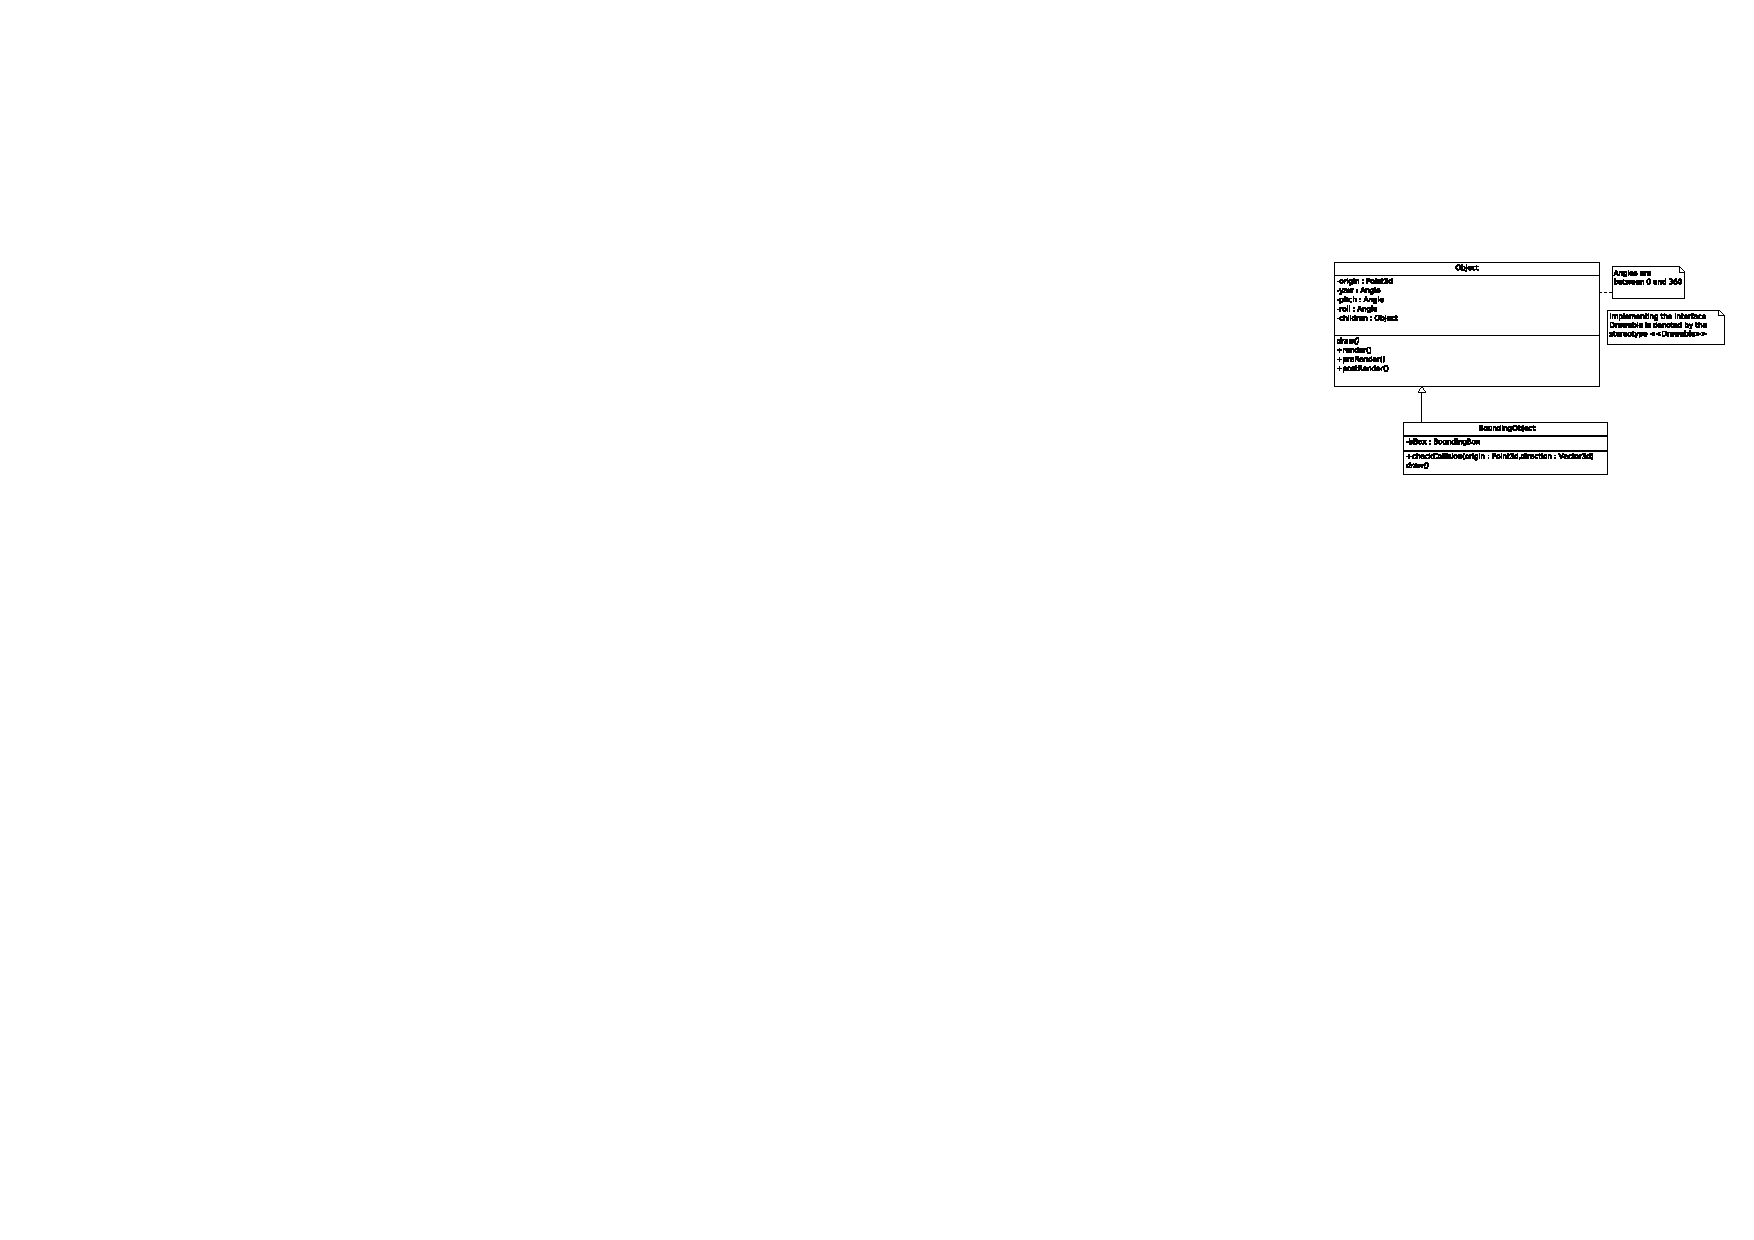
\includegraphics[width=0.9\textwidth]{../Class-diagram/Interfaces.pdf}
    	\caption{De verscheidene interfaces die ge\"implementeerd worden door klassen in het model van de sc\`ene}
    \end{figure}
    \label{app:Interfaces}
    \FloatBarrier
    \begin{samepage}
    \subsection{Communicatie klassen} \begin{figure}[h]
        \centering  	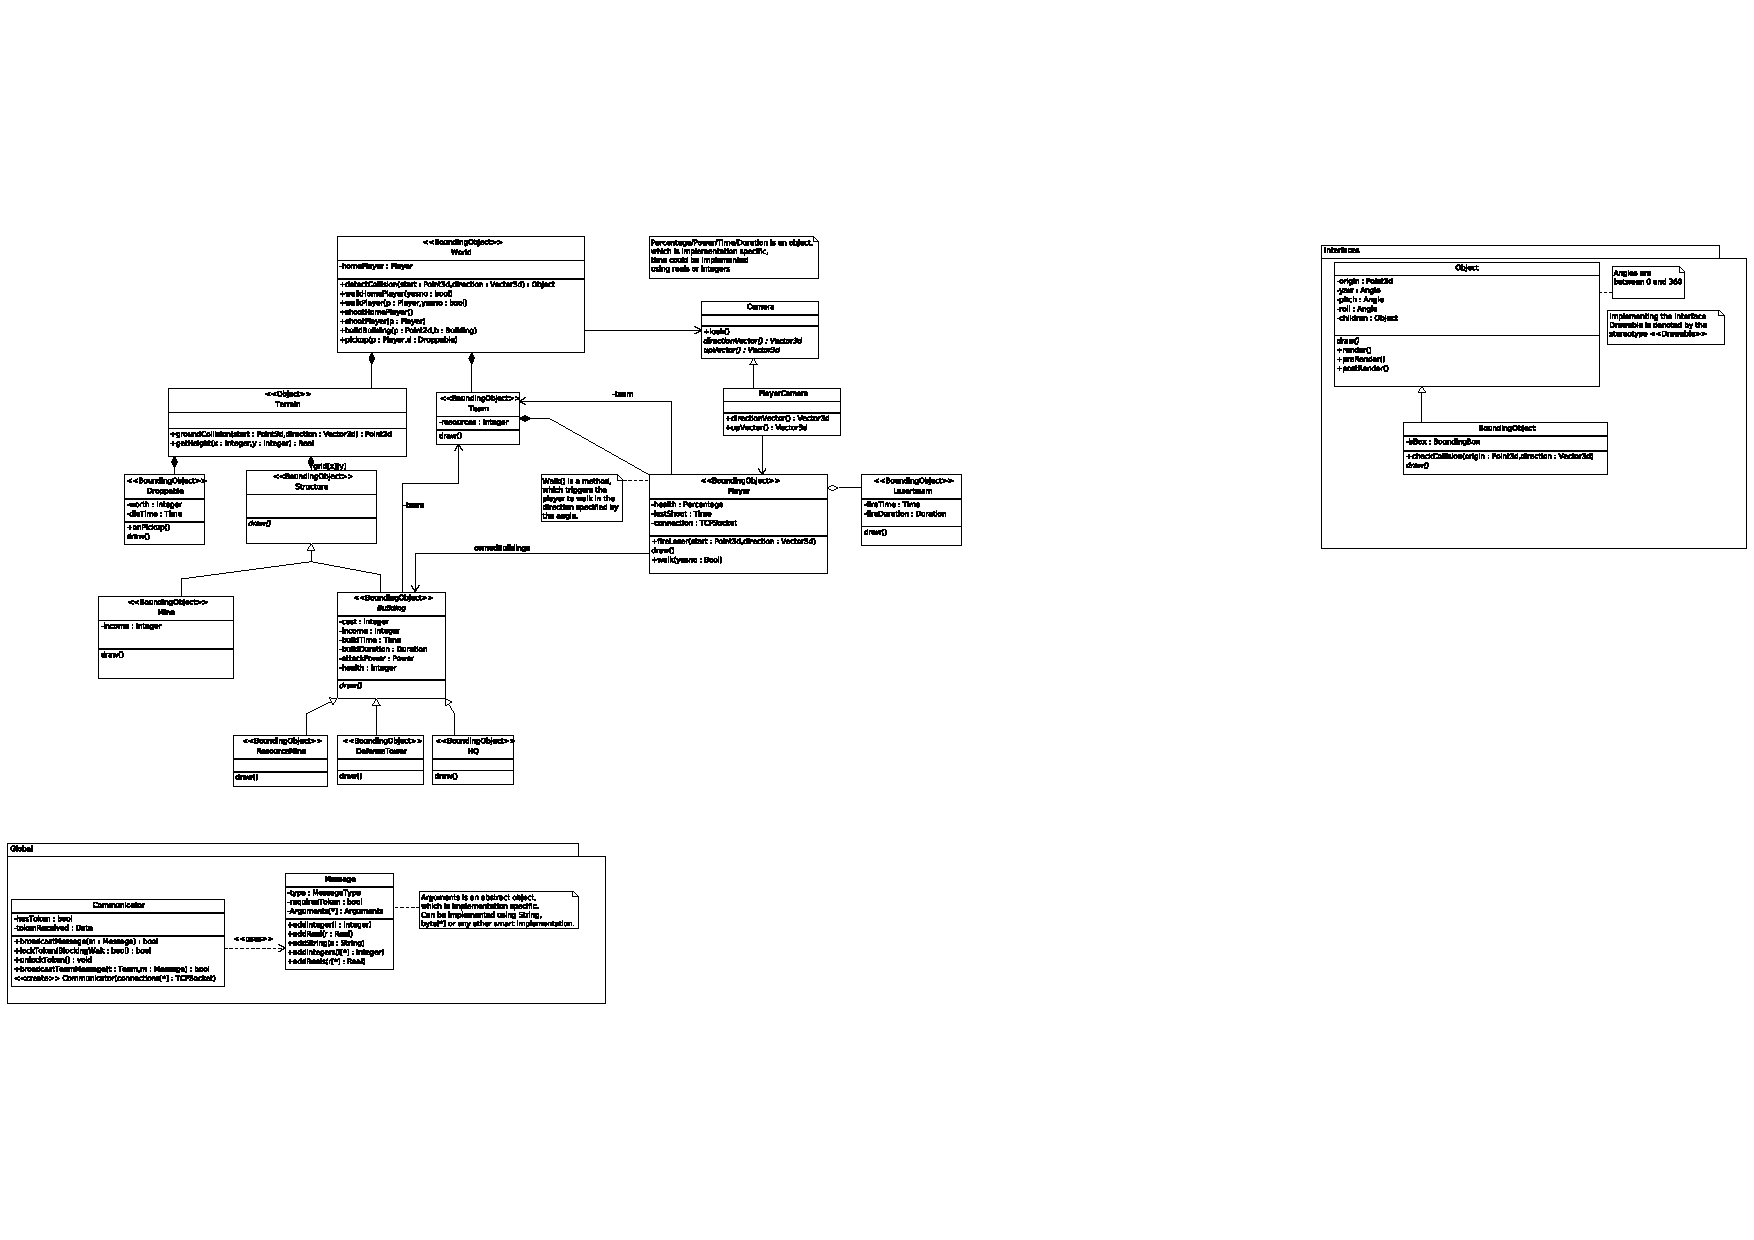
\includegraphics[width=\textwidth]{../Class-diagram/NetCommunication.pdf}
	\caption{De globale klasse die methoden verschaft om te kunnen communiceren met de medespelers.}
    \end{figure}
    \label{app:Comm}
    \end{samepage}
    \FloatBarrier
    
    
    \newpage
    
    \subsection{Klassendiagram voor de sc\`ene}
    \begin{figure}[h]
        \centering
    	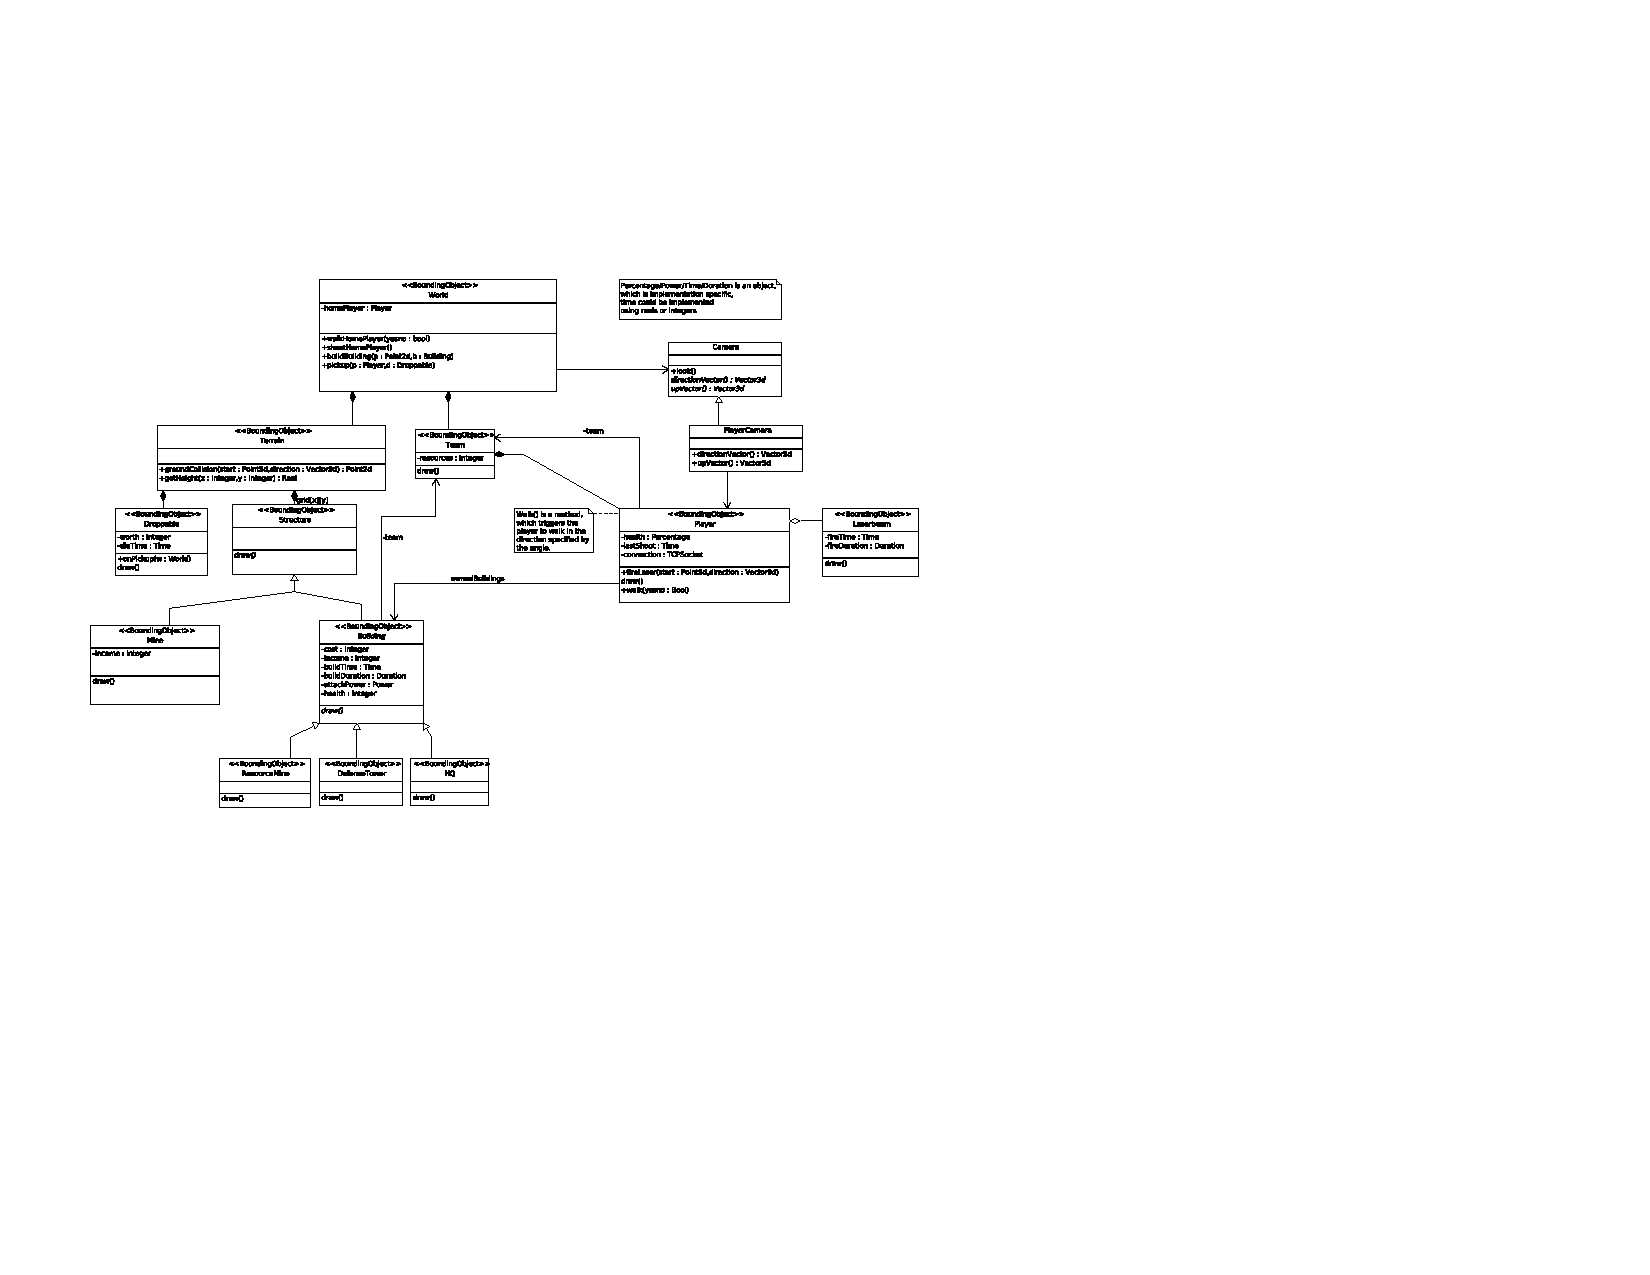
\includegraphics[angle = 90, height=0.95\textheight]{../Class-diagram/SceneModel.pdf}
	\caption{Het klassendiagram voor het model van de sc\`ene.}
    \end{figure}
    \label{app:Scene}
    \FloatBarrier
    \newpage
    
    \section{Voorbeeld van de interactie tussen de gebruikersomgeving en de protocolmodule}
    \label{sec:interactscenmodel}
    \begin{figure}[h]
    	\centering
	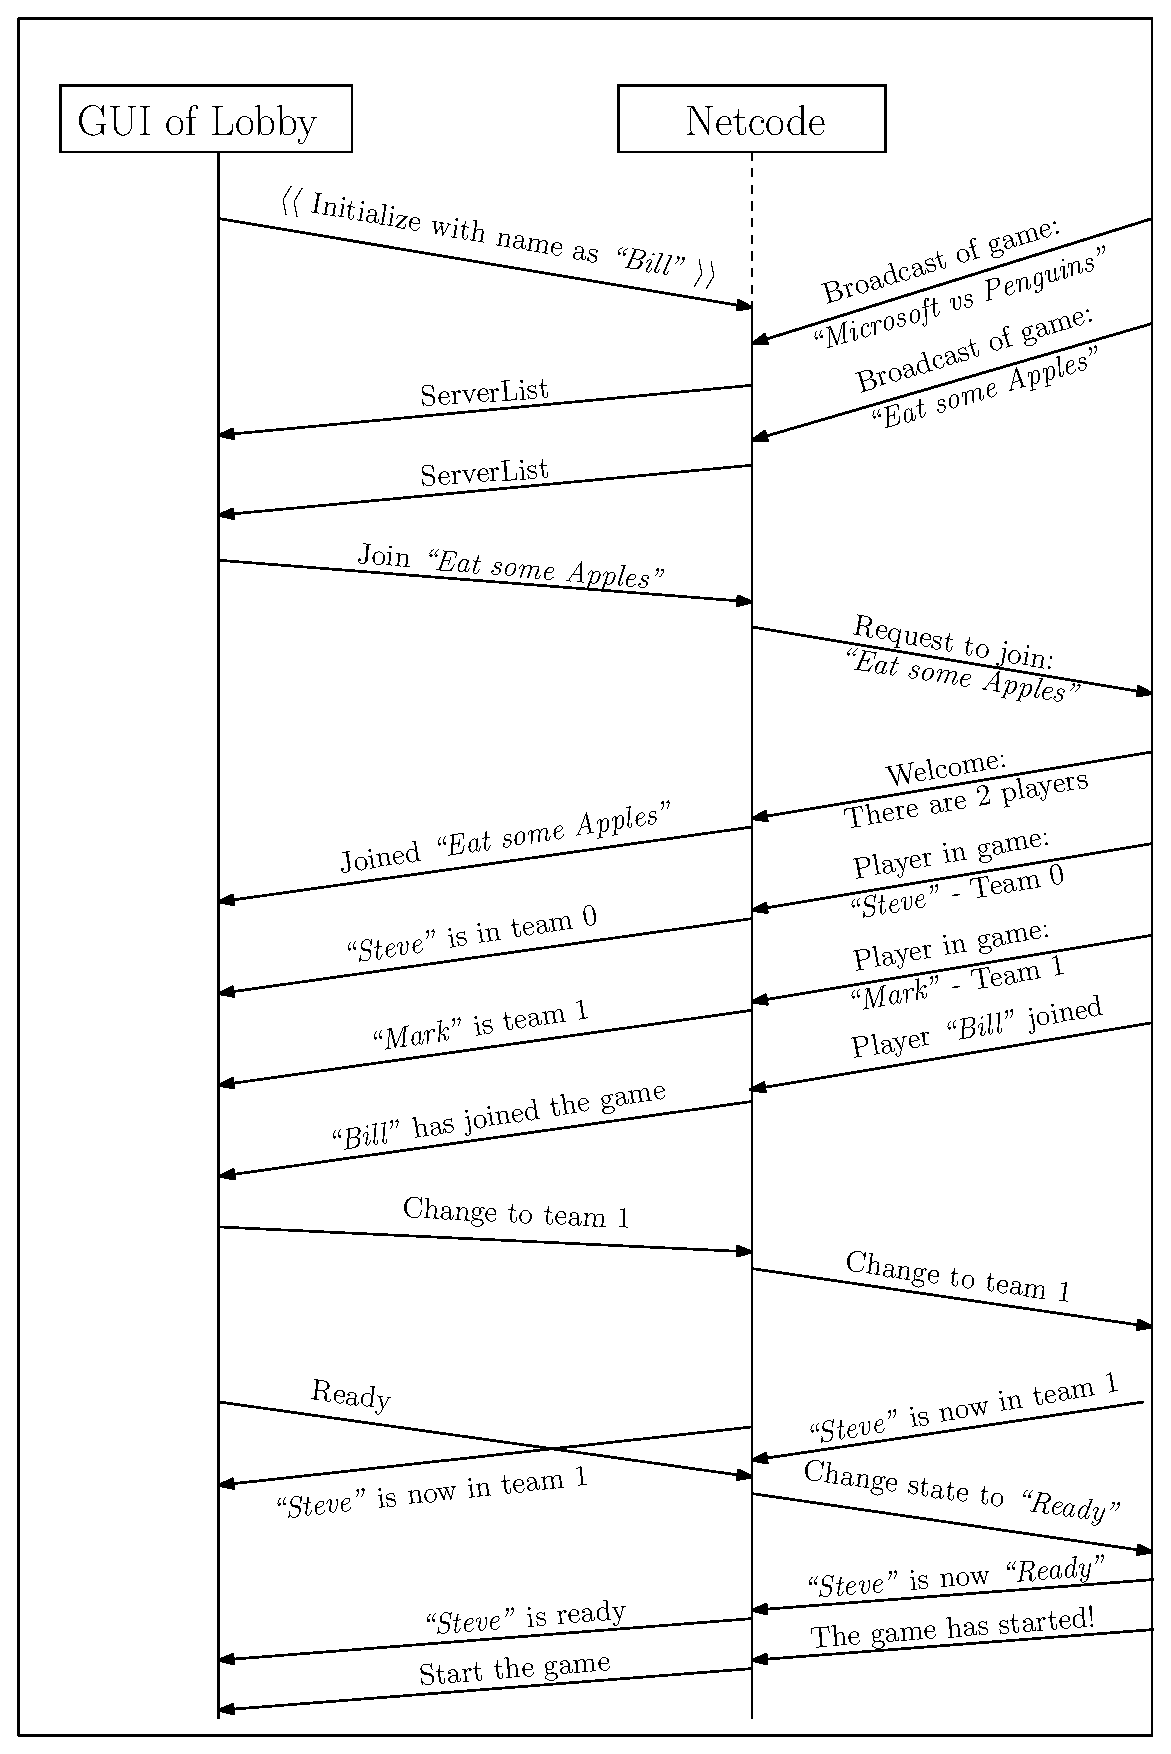
\includegraphics[height=0.7\textheight]{../Class-diagram/MSCLobby-console.eps}
	\caption{Voorbeeld van een interactie van de gebruikersomgeving en de protocolmodule.}
    \end{figure}
    \label{app:MSCLobbyCon}
    \end{document}